\documentclass[a4paper,10pt]{book}
\usepackage[utf8]{inputenc}
\usepackage[right=2.5cm,left=3cm,top=2cm,bottom=2cm,headsep=0cm,footskip=0.5cm]{geometry}
\usepackage[english]{babel}
\usepackage[T1]{fontenc} 
\usepackage{graphicx}
\usepackage{hyperref}
\usepackage{amsmath}
\usepackage{amsfonts}
\usepackage{amssymb}
\usepackage{color}


\begin{document}

\chapter{Characterization of analog ASIC for L1 Trigger decision}\label{cap.introduccion}
\pagenumbering{arabic} % para empezar la numeración con números
\section{CTA Trigger System}
%\Typical characteristics of trigger systems for IACTs, majority, sum, multilevel. Requeriments for LST. 
IACT's work detecting the Cherenkov light porduced by the interaction of gamma rays and other particles in the 
atmosphere. This cherenkov photons must be distinguished from those of the Night Sky Background (NSB) that fill 
the atmosphere. Telescopes are constantly receiving light from NSB, that could produce events in the detector,
together with the light produced by cherenkov showers. It is necessary to have a trigger system that analyzes 
the incoming light and takes the decision of storing the data of the showers and rejects the NSB events.\\
Usually this task is made by recognizing a concentration of signal from several pixels both in space and time. 
Showers are produced in a time window of a few nanoseconds, giving signal to a group of near pixels, while NSB light
is randomly distributed. Only when this coincidence of signal in time and space is produced, the trigger gives the 
instruction of storing the data.\\

There are two possible approaches for this detection of coincident light used in IACT's, called 
``majority trigger'' or ``sum trigger''. In majority trigger the light of each pixel is compared to a certain
threshold. If the signal of several (the majority of) pixels in a certain region exceeds the threshold in a brief time, 
then the trigger is fired. This approach presents a disadvantage when detecting low energy photon showers,
as happens in LST. The problem is that as the pixels must overcome the threshold individually, if the signal 
is too low, it's possible  that some of them won't exceed the threshold and therefore the event would be missleaded as a NSB event.\\

On the other hand, the sum trigger approach takes into account the signal coming to a group of several pixels. 
The light arriving to each pixel of the group is added and is this addition which must surpass a certain threshold to
fire the trigger. If several close group of pixels surpass the threshold at a given time window, then
the event is recorded as a shower event.\\

In the LST, a multilevel trigger system is used, that guarantees the rejection of the majority of the NSB light and 
satisfies the sensitivity required.\\

LST cameras have been designed to be modular  for several reasons of assembly and maintenance convenience. The pixels
in the camera are distibuted in 265 hexagonal modules of 7 pixels, that are connected to each of it's 6 neighbours.
The first trigger level (L0) sums the signal of the pixels in each module, and if it is significative, a trigger signal
is sent to the neighbours. In the second trigger level (L1), each module takes the trigger signal coming from its neighbours and 
compares it to a threshold to decide if the camera trigger is fired. Finally, the third level compares the camera trigger of
several telescopes and if two or more telescopes have triggered in a certain time window, the event is recorded. \\

\begin{figure}
\centering
 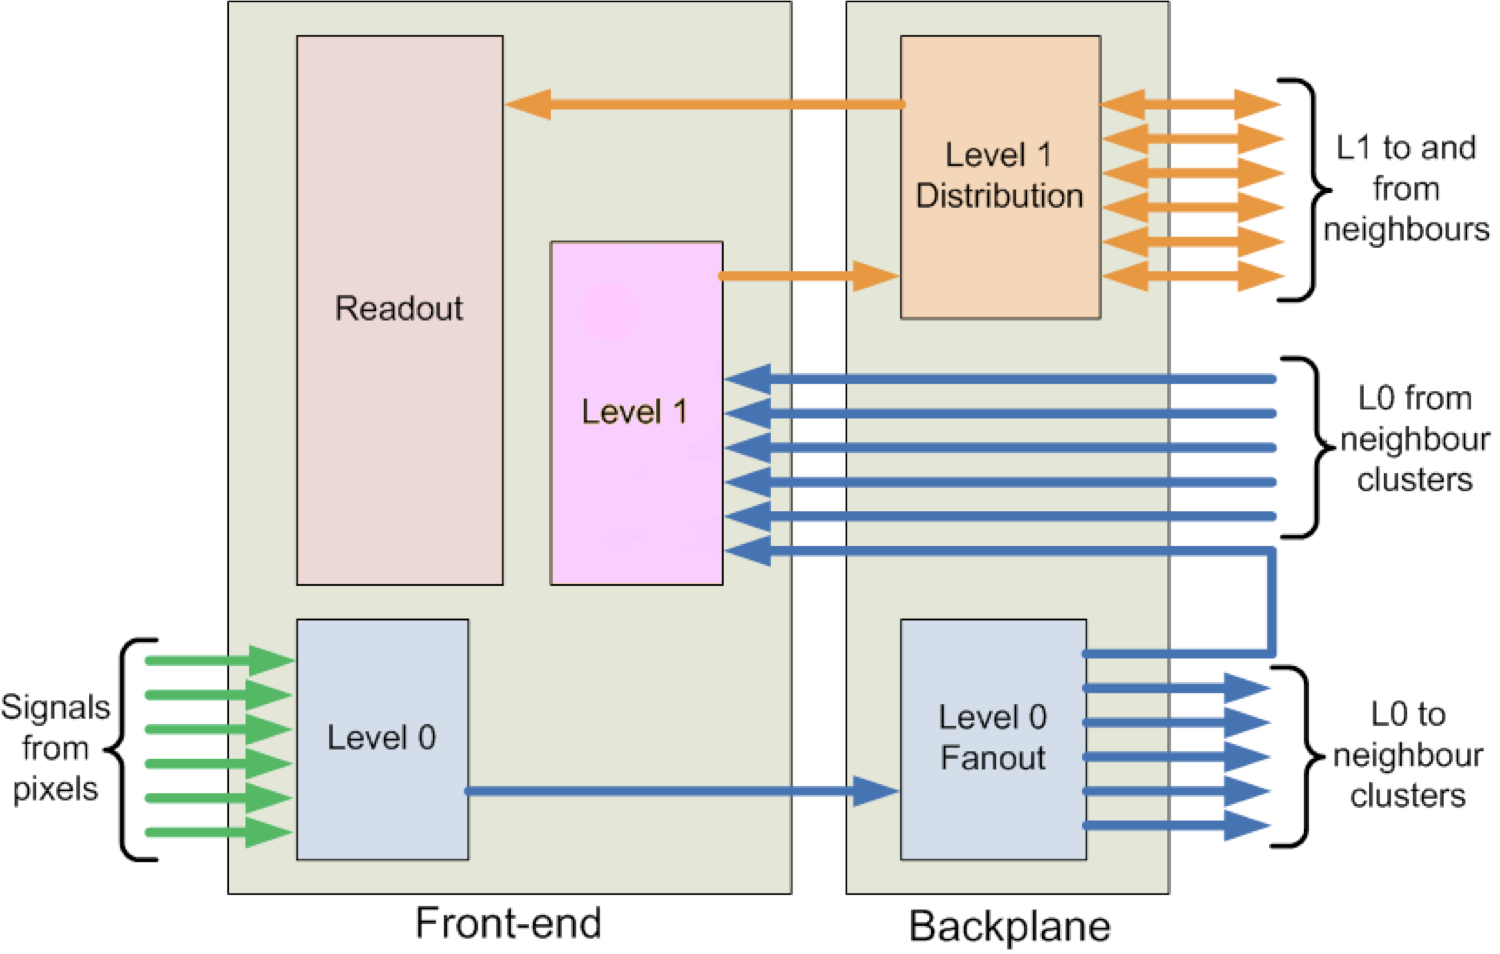
\includegraphics[bb=0 0 1296 675,scale=0.25]{./triggerscheme.png}
 % L1blockdiagram.png: 1296x675 pixel, 72dpi, 45.72x23.81 cm, bb=0 0 1296 675
  \caption{Architecture of the analog trigger system}
    \label{fig:trigger}
\end{figure}


\subsection{Pixel Level: L0 trigger decision}

The pixel level, dubbed for CTA as L0, takes into account the signals from the pixels in one module or cluster. If the trigger is fired, 
the signal is distributed by the L0 fan out to the local L1 and to the neighbours. 
Both, the majority and sum trigger approaches have been developed for  being used at the L0 trigger.

\subsubsection{Majority}

As explained before, the majority approach counts the number of pixels in a module that have a signal over a certain threshold voltage. 
When this happens, a digital signal is generated. The signal from all the pixels is added, resulting in a final signal with amplitude 
proportional to the number of activated pixels, that goes to the local L1 and the neighbour modules. This approach doesn't accounts for the number of photoelectrons that activated each pixel,
only for the number of pixels that have surpassed the threshold. This means that even if a large number of pixels in a region receives
a flash of light, if in each pixel the amount of photoelectrons is not enough, the event would be considered NSB and not recorded,
limiting the capacity of detecting low energy events. 

\subsubsection{Sum}

The sum trigger adds the signal received in each pixel of the module and the resulting signal is compared with a threshold voltage. If 
the threshold is surpassed, the signal is sent to local and neighbours' L1. This way makes it possible to take into account the contributions
of all pixels of the module, being able to reject NSB but also to improve the detection of low energy events. After adding the signals
of all pixels a clipping is applied to overcome afterpulse effects in the photomultipliers. Afterpulses are sometimes produced after a real pulse
in the photosensors, due to the ionization of residual gases, and can contribute with a very high amplitude to the sum. 

\subsubsection{L0 Fan-out}

The L0 signal must be distributed to the local L1 and the L1 of the neighbours. The L0 signal of each module is replicated seven times, 
one of them is sent to the local L1 and the rest to the neighbouring modules. 

\subsection{Camera Level: L1 trigger decision}

Camera level trigger decision system, in CTA named L1, analogically adds the resulting signals of L0 trigger from neighbouring modules and compares 
the result with a threshold voltage. If the analog sum is over the threshold, a signal is sent to the L1 distribution to trigger
the camera. 
Each module has six neighbours from which it receives the L0 signals from L0 fan-out, plus the local L0, there are seven
signals that can be combined. To ensure that all modules are paricipating in the trigger and addings are made in an efficient way, it is possible
to configure by slow control different modes where intelligent configurations of neighbouring signals are added. In figure~\ref{fig:trigmodes} the three modes,
named 2, 3 and 4, are shown. This configurations make it possible, through combinations of two, three or four modules, to evaluate
any trigger region. 

\begin{figure}
\begin{center}
 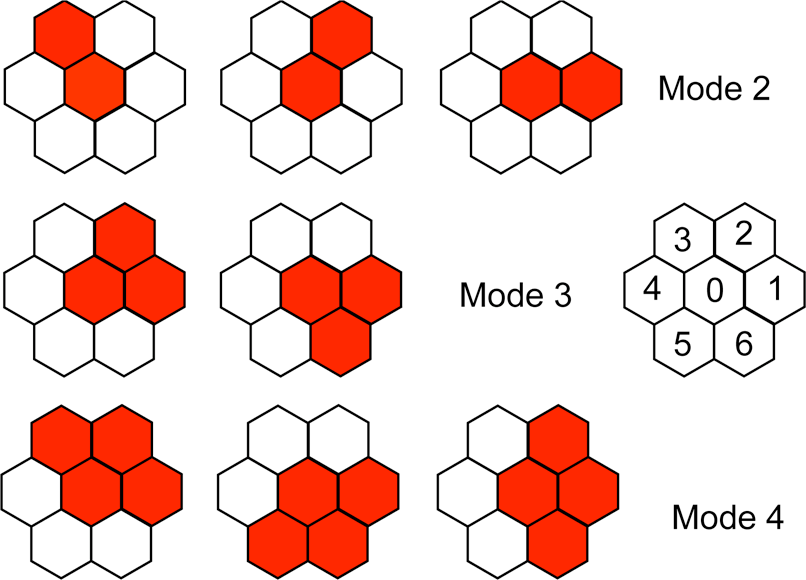
\includegraphics[bb=0 0 1296 675,scale=0.25]{./triggermodes.png}
 % L1blockdiagram.png: 1296x675 pixel, 72dpi, 45.72x23.81 cm, bb=0 0 1296 675
  \caption{Illustration of the three possible modes for adding signals of neighbouring modules. Each hexagon represents a group of seven photomultipliers.}
    \label{fig:trigmodes}
\end{center}
\end{figure}

\subsubsection{L1 Trigger Distribution}

The L1 trigger distribution system allows the L1 signal to reach the data adquisition systems of all the modules and start the digitalizing 
process. Every module can send the L1 signal to its six neighbours, and is awatred of its position in the camera. This way, when a module receives
a L1 signal, it can be delayed depending on the position in the camera and be sent to the appropriate neighbours following the preconfigured paths. (See figure ~\ref{fig:trigpaths}). The distribution paths are firmware configurable and they can automatically be reconfigured to go through the full 
camera, even if for some reason one module is malfunctioning.

\begin{figure}
\centering
 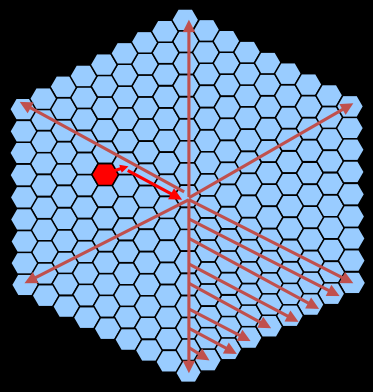
\includegraphics[bb=0 0 1296 675, scale=0.5]{./triggerpaths.png}
 % L1blockdiagram.png: 1296x675 pixel, 72dpi, 45.72x23.81 cm, bb=0 0 1296 675
  \caption{Paths for trigger distribution over the entire camera.}
    \label{fig:trigpaths}
\end{figure}

\subsection{Array Level trigger decision}
Array level trigger looks for coincidences in events recorded by several telescopes. If more than one telescope has a camera trigger in
a certain time window, it is likely that the light is produced by a cherenkov shower, so the data is stored. This level allows to reject
the majority of NSB events that have overcomed the lower level triggers. 

\section{Analog ASIC for L1 Trigger System of LST camera}

For the implementation of the analog L1 Trigger System on CTA cameras, an Application Specific Integrated Circuit(ASIC) was developed (reference).\\

The function of the ASIC is to collect the analog signals from the L0 fan-out, add them in three different configurations and discriminating
the resulting voltage in order to produce digital trigger output signals.\\

The ASIC was designed to accomplish several specifications needed to ensure the required performance for CTA. The ASIC must be flexible in order
to work with the two L0 approaches (sum and majority) and also to configure the three modes named in previous section. The noise must be lower than 
0.2 photoelectrons per added channel. The range of the signals processed must be between 0.2 and 100 phe. The gain of the ASIC must be
such that will avoid saturation if the entire signal is concentrated in one channel. Bandwidth must be greater than 500MHz to avoid NSB
pulses being added with the signals. As long as for CTA cameras all the electronics are installed inside the camera box, the ASIC must be compact
and have a low power consumption $(< 150 mW/ch)$.\\

The scheme of the reconfigurable ASIC is shown in~\ref{fig:figure1}.\\

\begin{figure}
\begin{center}
 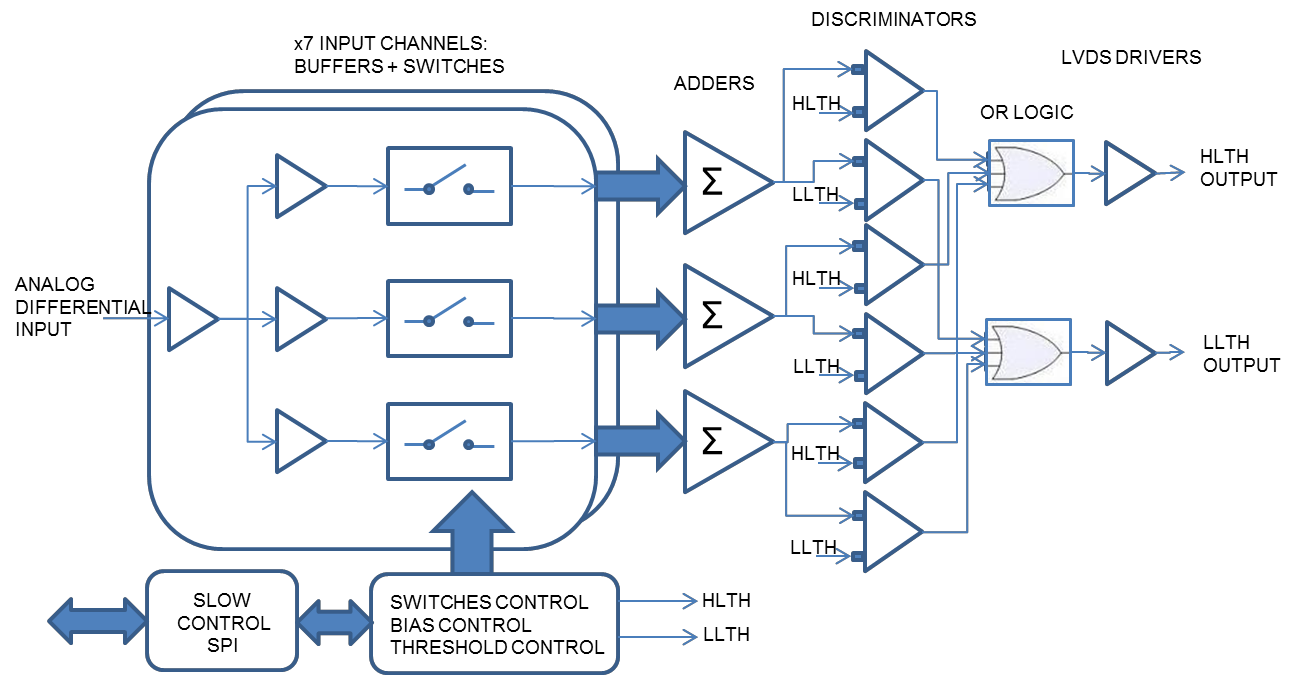
\includegraphics[bb=0 0 1296 675,scale=0.25]{./L1blockdiagram.png}
 % L1blockdiagram.png: 1296x675 pixel, 72dpi, 45.72x23.81 cm, bb=0 0 1296 675
  \caption{L1 ASIC Block diagram}
    \label{fig:figure1}
\end{center}
\end{figure}

There are seven input differential analogue channels and two output differential digital channels.
The seven signals arriving the input channels are replicated three times and sent to three analogue adders (dubbed A, B and C). The signals
that are sent to each adder are selected by a set of switches, corresponding to the different configurations of the three modes.
The output of the adders are sent to two groups of discriminators, which makes the comparison of the added signal with a threshold voltage.
The two discriminators have a different and independent threshold voltage, low level and high level threshold, generated by differential DAC's. 
The discriminator outputs are connected to two OR gates which are in turn connected to Low-Voltage Differential Signalling (LVDS) transmitters 
that provide the trigger signal. 


\section{Characterization of the ASIC}

About ~400 asics where produced and quality control tests were performed to check their functioning. The quality control tests probed 
several characteristis of the ASICs, such as gain, noise and offset, for all the channels, adders and discriminators. From all the ASICs
tested, 389 surpased the quality control and the results of their tests where analyzed to characterize the performance of the ASIC. 
Averaging to all the ASIC analyzed, the result is an overall view of the features that a default ASIC would have. To obtain the gain
and offset of the ASIC a fitting method was used with the data of the Rate Scan procedure performed during the tests. 

\subsection{Quality Control Tests}
\label{subsec:qatest}
The quality control tests were made at the electronics laboratory at CIEMAT and consisted of several checks that evaluated
the performance of the different parts of the ASIC (seven input channels, three adders and two LVDS outputs).

\subsubsection{Set Up}

Preguntar a Gustavo sobre el setup y describirlo aqui. 

\subsubsection{Test DAC}

Measurement of the maximum and minimum voltage of the DAc's (it is possible to know the range of the 6 DAC's) directly from the output pin
of the ASIC by a Multimeter. Each DAC is composed by a 2 DAC's of 9 bits (Positive part P and negative part N) to get a final resolution of 10 bits. To measure
this it is set the code in the register with the maximum values of the Positive part (P), the minimum value of P and the same with Negative part (N).

\subsubsection{Voltage Test: Rate scan}

The Voltage test measured the gain of all seven input single channels and the two outputs for 10
different voltages (from 100mV to 1000mV) using a rate scan methodology, consisting on the
comparison of the input trigger rate from a generator on the evaluation setup and the ASIC trigger
output rate. This computation is performed with scalers implemented in the FPGA board.

\subsubsection{Test Adder Channels}

The gain of different sum combinations obtained by the same rate scan methodology. There are 3 different methods combining different
chanels of different adders.

\subsubsection{Analog Offset test}
The Analog offset test consisted in the measurement of the offset in the Analog Adder Output test,
which is the output of a multiplexor that selects among the available analog output adder, plus a
buffer for the output pins. The measurement is directly from the differential output pin of the ASIC
by a Multimeter.

\subsubsection{Digital Offset test}


The Digital offset test procedure was the measurement of the offset in the LVDS digital outputs, 0
and 1, by the evaluation of the outputs status as a funtion of the threshold.
The methodology consist on increasing the threshold from 0 Volts using the DAC's values until find
the minimum value that the output crosses from 1 to 0, and the maximum cross from 0 to 1. The
voltage between this two points is the noise of the digital output, and the mean point is the offset.
Setting the Threshold to 0 it is possible 3 different behaviors:
If the status of the digital output is always a logic "1" (tagged as type "Pos") it is possible tomeasure the minimum and the maximum points and therefore it is possible to calculate the Offset
and the noise.
If the status of the digital ouput is always a logic '0' (tagged as type "Neg"), it is not possible to
measure neither the minimum nor the maximum point, and then a value of zero is assigned by the
program both to the noise and the offset.
Finally, if the status of the digital ouput is switching (tagged as type "Com"), it is only possible to
measure the maximum value, and the other is assigned to 0. In this case the noise is
understimated and the threshold is overstimated.

\subsection{Quality Control data analysis}

The quality control provided a datasheet for each individual ASIC with the results of the tests which where analyzed to charanterize the manufactured ASICs. Each combination of channel (7), adder (3) 
and discriminator(2) is accounted separately, having a proper gain, offset and noise. This procesure allows the detection of outliers that could mean a defect in a part of the ASIC.
The quality control tests provided direct measures of  offset and noise, but gain must be calculated from the rate scan results in the test voltage. This procedure also gives other way of measuring the offset. 
The computation of gain and offset from the Rate Scan, explained in the next section, was perfomed considering a linear behaviour of the input voltage vs. voltage of the 50\% trigger rate. From a linear fit, the gain and offset 
are obtained.   

\subsubsection{Fitting Rate Scan}

In figure~\ref{fig:linearfit} the rate scan result versus ten input voltages for a certain path of one ASIC is plotted. The linearity can be easily appreciated, specially for low input voltages (under 500 mV).
If we assume a linear model, the relation between the input voltage and the rate scan result should be:

\begin{equation}
\label{eq:fit}
V_{rs} = Gain*V_{input} + Offset
\end{equation}


\begin{figure}
\centering
 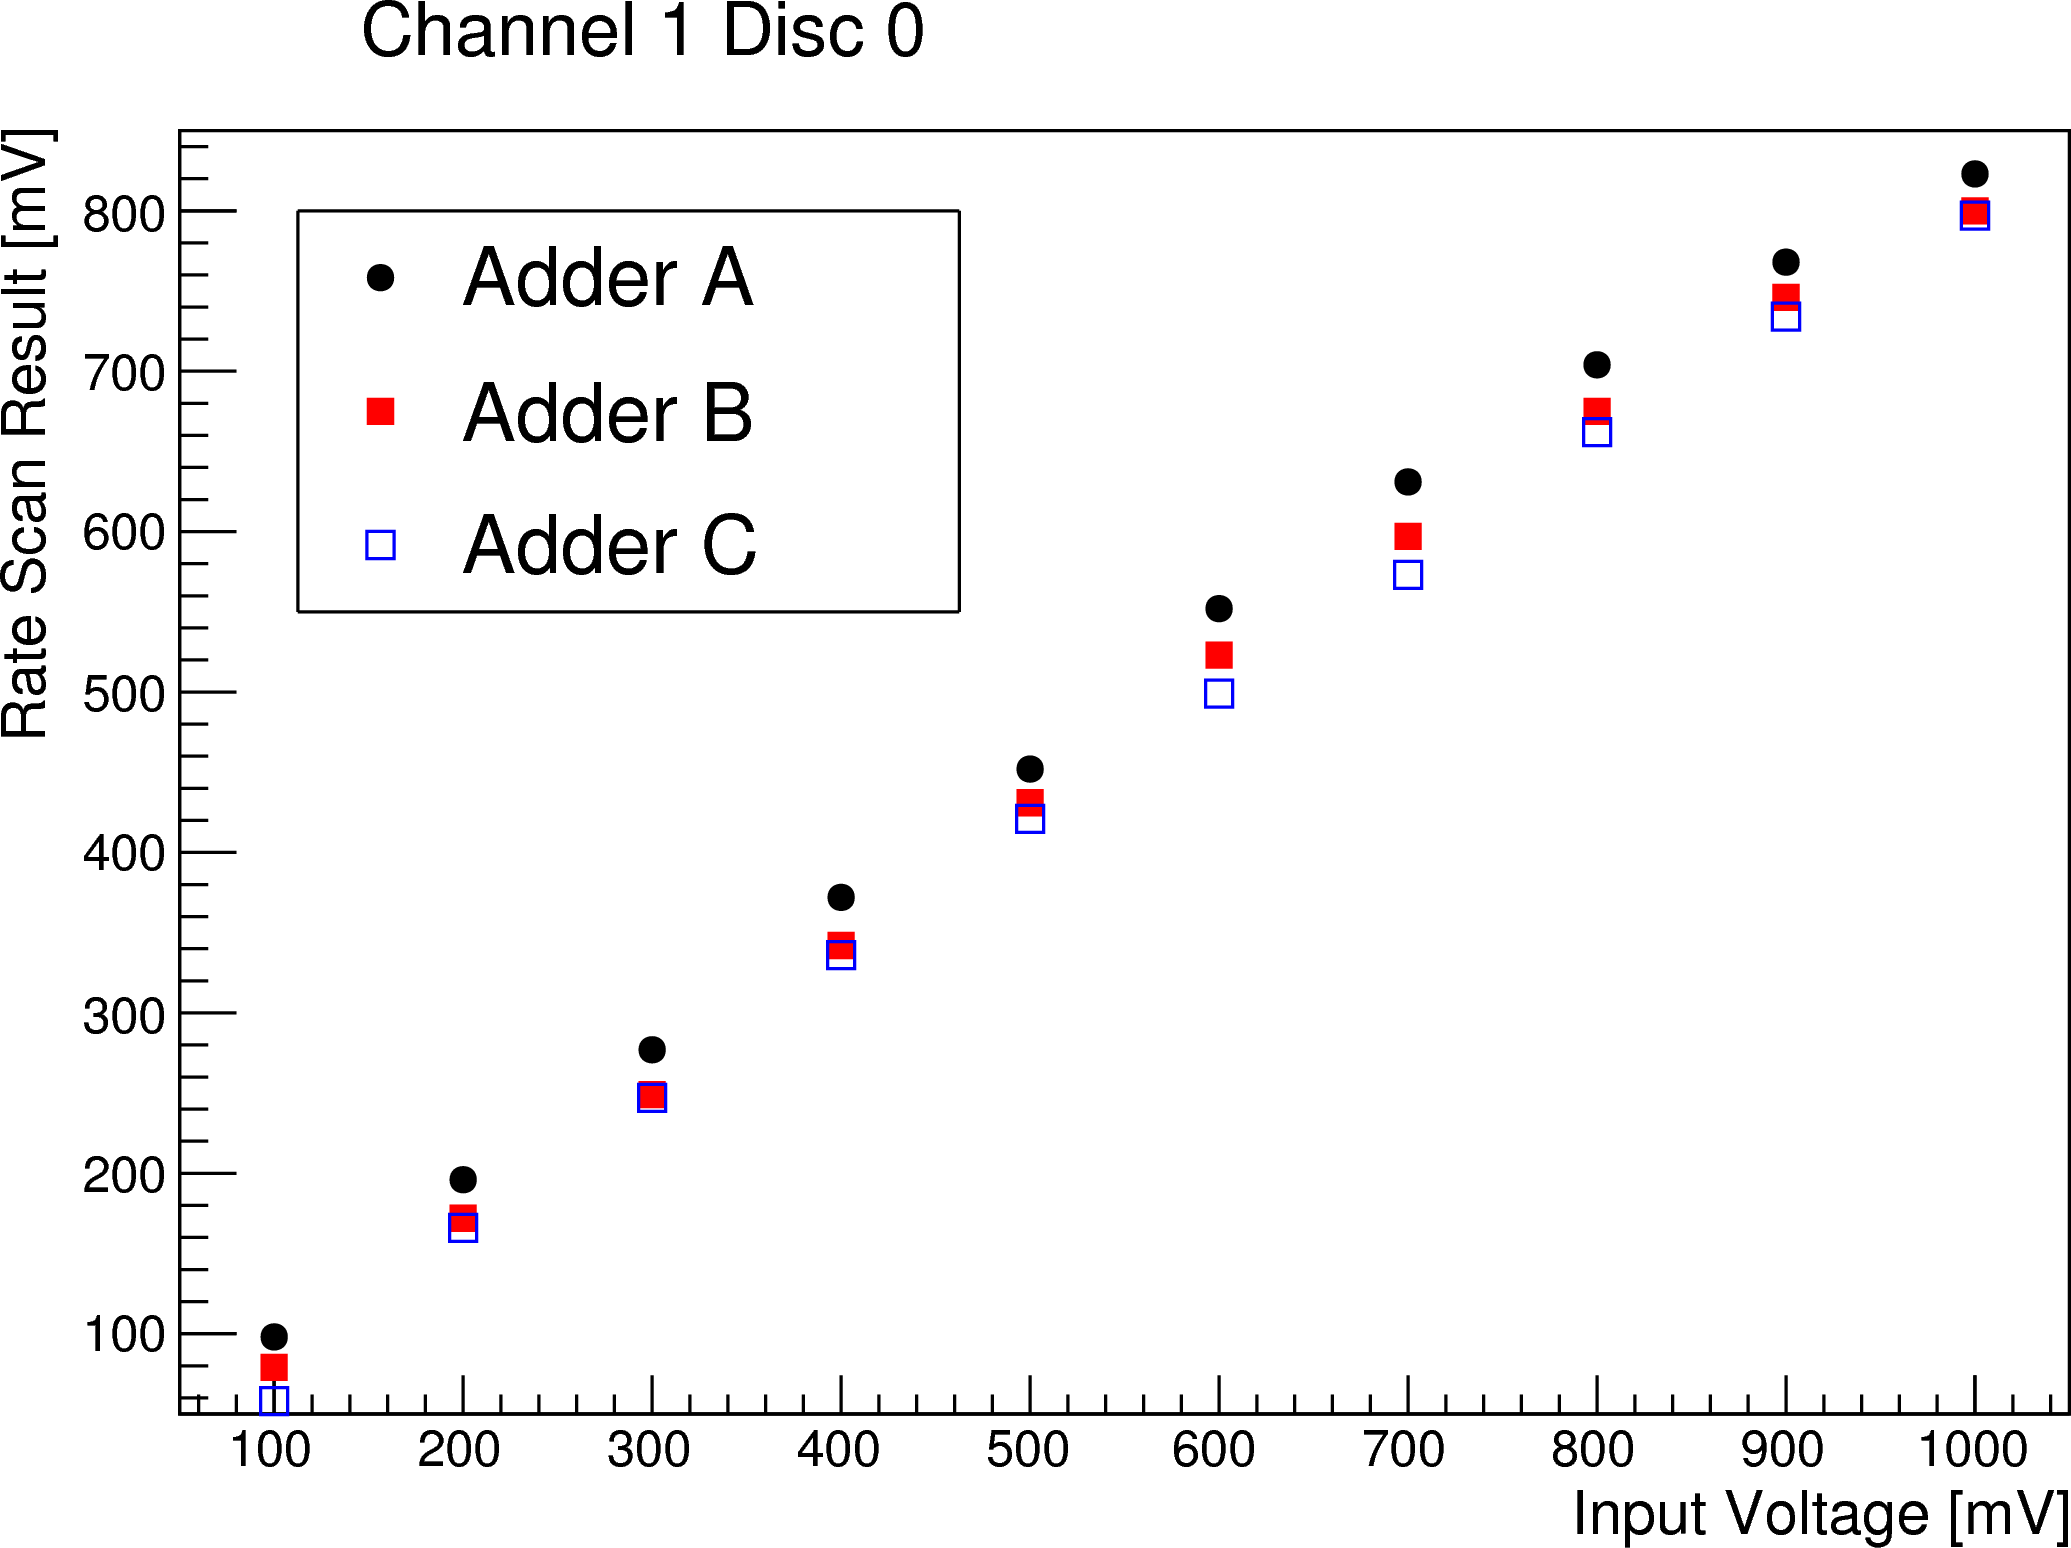
\includegraphics[width=0.5\textwidth]{./linearfit.png}
 % linearfit.png: 2071x1548 pixel, 300dpi, 17.53x13.11 cm, bb=0 0 497 372
  \caption{Rate scan result from one of the voltage tests for ASIC \#61. It can be observed a linear tendency which deteriorates at high voltages. 
  Similar plots where obtained from the rest of channel-adder-discriminator combinations. }
    \label{fig:linearfit}
\end{figure}

Where $V_{rs}$ represents the threshold voltage that gives a rate of 50\% trigger, and $V_{input}$ is the input voltage. The use of this method has the advantage of obtaining not only
the gain but also the offset of the ASIC without having to measure it with a multimeter. 
Since linearity seems to depend on the input voltage, is necessary to consider a range for the fitting where the linearity is better. To do so, several ranges were fitted and the offset obtained
was compared to the offset measured with the multimeter in the analog offset test. The range where the difference between the two offsets was lower should be the best range
to fit the linear model. The resulting range was the lower input voltage possible, from 0 V to 300 V and so this range was used to calculate the gain and 
offset for every path of each ASIC. 


\subsection{Characterization: Procedure}

In the next sections the characterization of the gain, offset and noise of the ASICs analyzed is commented. Some outliers with low gains are identified and also the adders are confirmed as the responsible element 
on introducing the measured offset.

\subsubsection{Gain}

The gain was caclulated with the model fitting decribed in the previous section. Figure~\ref{fig:gaindist} shows the distribution os gain values over the paths of the 389 asics. A clear gaussian profile is observed, 
centered in the characteristic gain of 0.87, the expected result according to the design specifications. Some outliers were identified having gain values that are too low for the requisites of the ASIC, 
which could signify a malfunctioning in the ASIC. Fitting the histogram to a gaussian, it is possible to see that the probability of an ASIC to have a gain lower than 0.7 in any of its paths is lower than 0.025\%.
There are also some outliers with higher gain values, but the probability of any entry to have a gain over 1.05 is lower than 0.007\%. The outliers are identified in image~\ref{fig:gaindist} by is ASIC number.
\\
\begin{figure}
\centering
 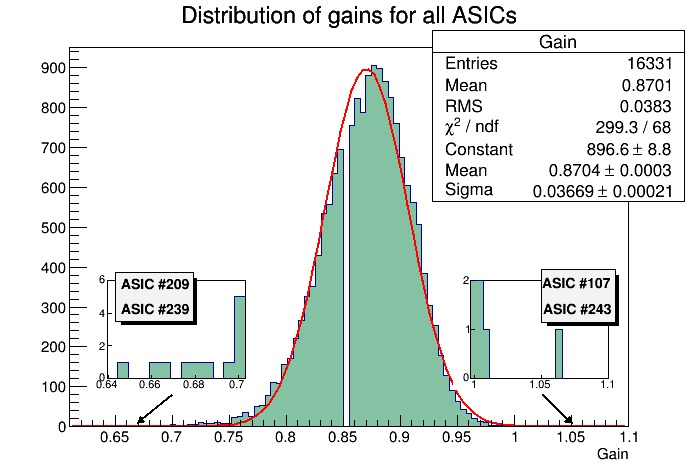
\includegraphics[width=0.8\textwidth]{./gaindistribution.jpg}
  \caption{Distribution of gains for all ASICs. Each entry represents the gain of one possible path (combination of channel-adder-discriminator). The red line represents a gaussian fit with mean 0,8704 and sigma 0,3669. 
  The zoom-ins show several outliers with gains very deviated from the average. }
    \label{fig:gaindist}
\end{figure}

Cleaning the outliers from the sample, the characteristic gain is $0.87 \pm 0.038$, obtained from the gaussian fit. This is an average to all the possible paths of channel, adder and discriminator in the ASICs
analyzed. A single path characterization can be consulted in table (ANEXO), each entry averaged to all ASICs. 
When obsserving the average gain for each channel separately in table~\ref{tab:gainch}, and in image (TAL) it can be observed that the second channel has a slightly lower gain than the others,and the third one a slightly higher gain. 
This effect comes out from the configuration used during the quality control tests. The third channel was connected directly to the pulse generator, while the second channel had to be fed
with a cable of different length than the others. 
\\\\
\begin{table}
\centering
\begin{tabular}{l|l|l|l}
Channel & Mean Gain & RMS \\\hline
1 & 0.871 & 0.035 \\
2 & 0.839 & 0.036 \\
3 & 0.880 & 0.036 \\
4 & 0.873 & 0.036 \\
5 & 0.876 & 0.036 \\
6 & 0.873 & 0.036 \\
7 & 0.878 & 0.036 \\
\end{tabular}
\caption{\label{tab:gainch} Mean gains for the seven channels, averaged to the sample of all asics, without the outliers.}
\end{table}

\begin{figure}
\centering
 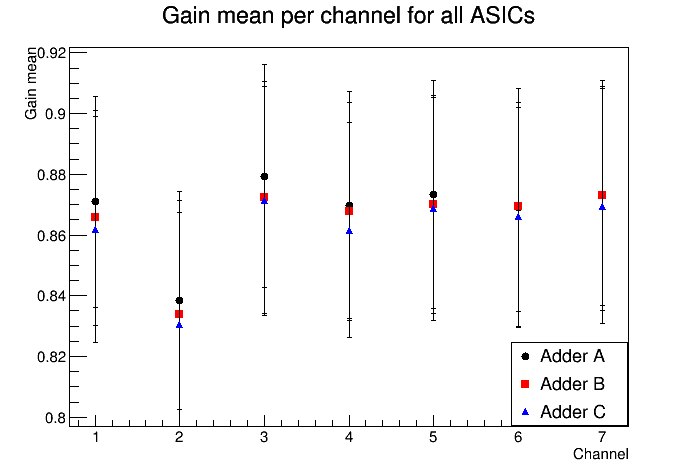
\includegraphics[width=0.6\textwidth]{./gainschannel.png}
  \caption{Distribution of gains for all ASICs. Each entry represents the gain of one possible path (combination of channel-adder-discriminator). The red line represents a gaussian fit with mean 0,8704 and sigma 0,3669. 
  The zoom-ins show several outliers with gains very deviated from the average. }
    \label{fig:gainch}
\end{figure}

To find if any part of the ASIC is dominating the fluctuations of the gain, correlation plots between channels, adders and discriminator were studied. A remarkable correlation is not observed in any
of the elements of the ASIC, so we can conclude that all parts contribute to the final value of the gain in a similar way. 


\subsubsection{Offset}

The offset has been measured in three different ways. In the tests, the analog Offset was directly measured with a multimeter, the digital Offset was measured using the procedure described in section~\ref{subsec:qatest},
and finally, from equation~\ref{eq:fit} an Offset value that will be so called Fit Offset was obtained.\\

In figure~\ref{fig:offsetdist}  the distribution of the analog and digital offsets are shown. It must be noted that it was not possible to measure the digital offset for all the configurations, only the ones with an output 
status tagged as ``Pos'', so it's not possible to measure negative values of digital offset. Some outliers were detected, with digital offset values very deviated from the mean, which has been removed from the sample at the final characterizaton. Those outiers correspond to ASICs 110,
209,248 and 437.\\\\
\begin{figure}
\centering
 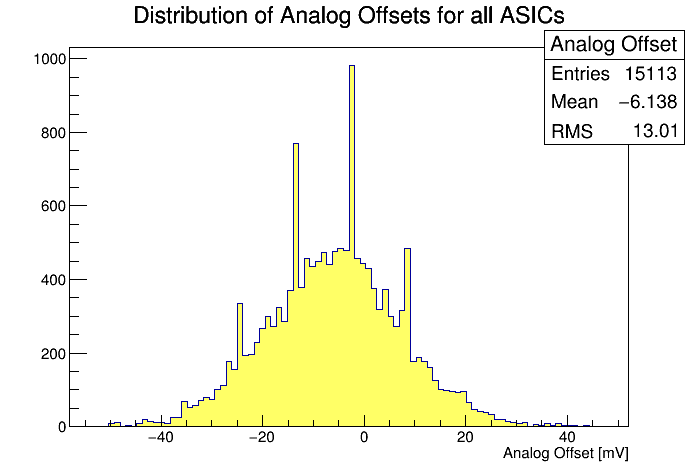
\includegraphics[width=0.6\textwidth]{./analogdist.png}
  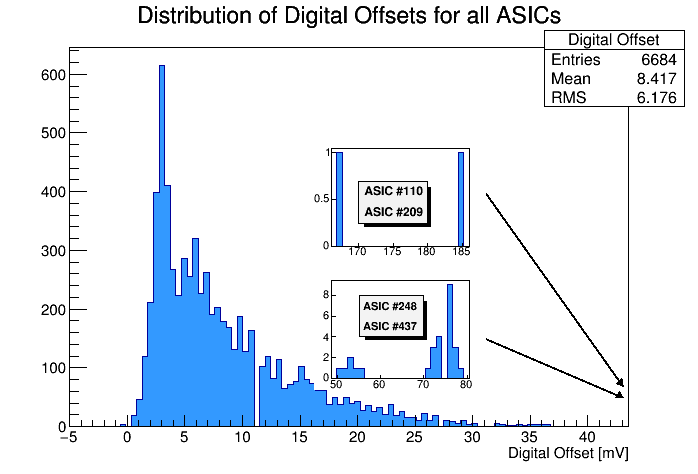
\includegraphics[width=0.6\textwidth]{./digitaldist.png}
  \caption{Distribution of offsets for all ASICs. Each entry represents the gain of one possible path (combination of channel-adder-discriminator).\textit{Top:} Analog offset. \textit{Bottom:}
  Digital offset. The zoom-ins represent outliers in the digital offset.  
  The zoom-ins show several outliers with gains very deviated from the average. }
    \label{fig:offsetdist}
\end{figure}

The averaged value of the analog offset is $-6.138 mV$ with RMS of $13.01 mV$ while for the digital offset the mean is $8.41mV$ with RMS of $6.17 mV$. Plotting the correlation between the two measured offsets(~\ref{fig:offsetcor} it can
be seen that there is a correspondence between the two ways of measuring the offset.

\begin{figure}
\centering
 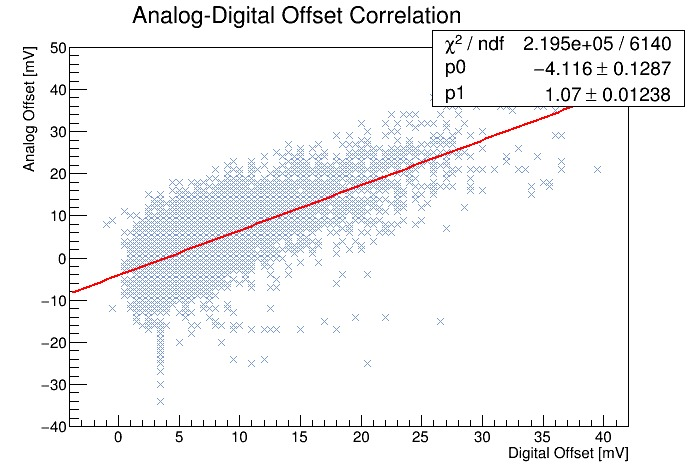
\includegraphics[width=0.5\textwidth]{./offsetscor.jpg}
  \caption{Correlation between values of the analog offset and the digital offset measured in the quality control test.}
    \label{fig:offsetcor}
\end{figure}

Regarding the fit offset, the distribution of the obtained values is shown in figure~\ref{fig:fitoffdist}. To check the validity of this method of obtaining the offset value, the difference between the fit offset and
the analog offset has been studied.  The averaged value of the fit offset is $0.1334 mV$ with RMS $13.75 mV$. The mean difference between the analog offset and the fit offset is of $5.55 mV$ with RMS $8.06 mV$.
\\
\begin{figure}
\centering
 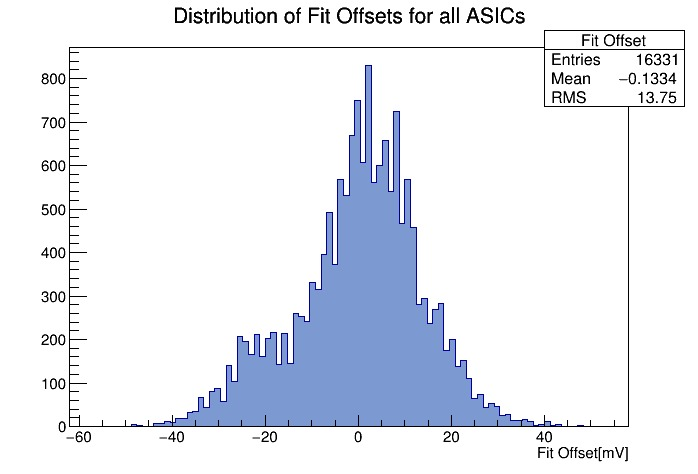
\includegraphics[width=0.4\textwidth]{./fitoffsetdist.jpg}
  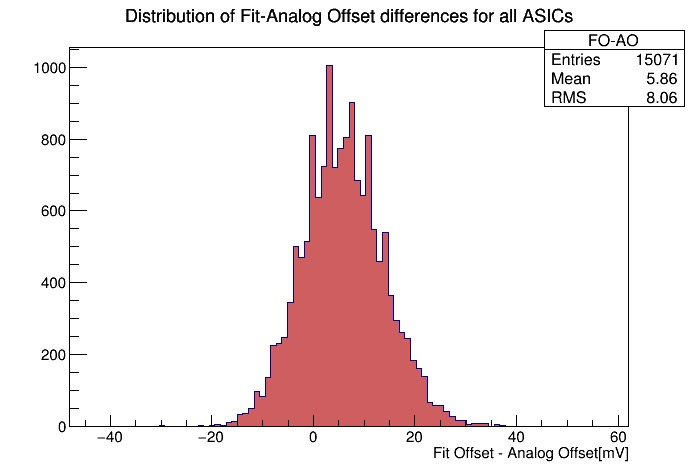
\includegraphics[width=0.4\textwidth]{./diffoffsetdif.jpg}
  \caption{\textit{Left:}Distribution of offset calculated from the model fitting. \textit{Right:} Distribution of the difference between the analog offset and the fit offset.}
    \label{fig:fitoffdist}
\end{figure}

Checking the correlation between the two offset values (fig~\ref{fitoffsetcor}) it can be observed that even there is a clear correlation between them, a factor relating them must be missing, and the fit offset is underestimating the analog offset. 
\\
\begin{figure}
\centering
 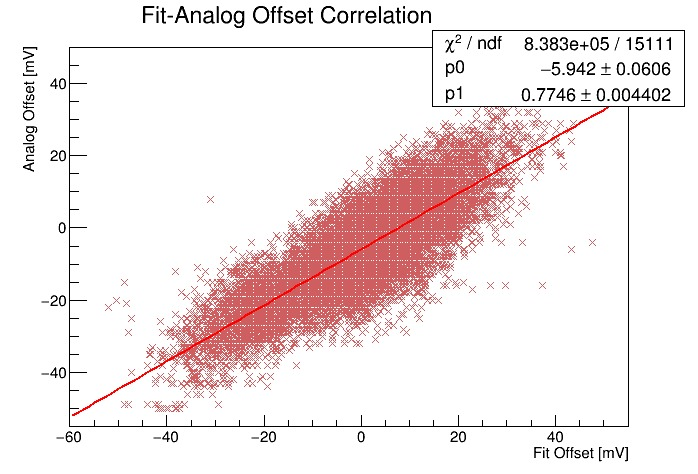
\includegraphics[width=0.5\textwidth]{./fitanalogcor.jpg}
  \caption{Correlation between the analog offset and the fit offset.}
    \label{fig:fitoffsetcor}
\end{figure}

In figure~\ref{fig:offch} the averaged offsets to all ASICs, separated by channels and adders are plotted. In general the offset takes similar values for all the channels and adders, without any remarkable outlier.
In table (ANEXO) the average offsets to all ASICs in every single path are presented, as a general characterization of what is considered a typical ASIC. 
\\

\begin{figure}
\centering
 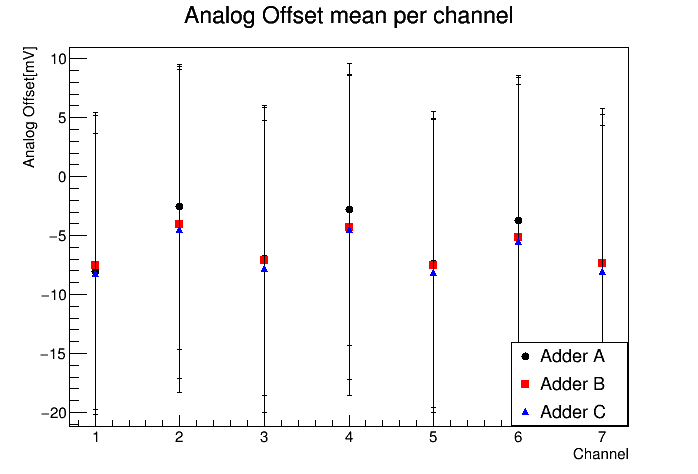
\includegraphics[width=0.4\textwidth]{./analogch.png}
  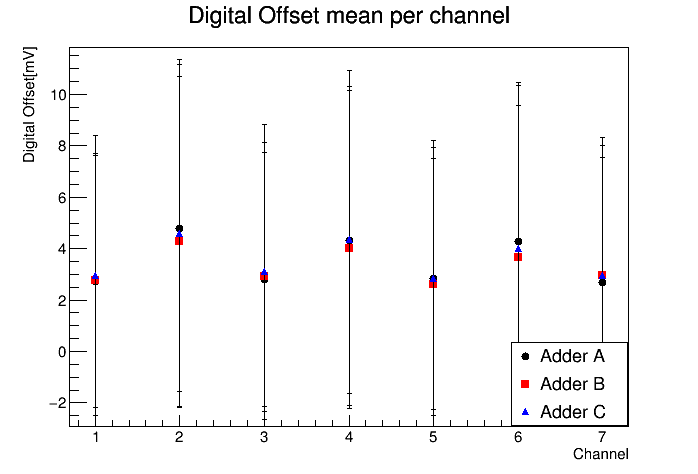
\includegraphics[width=0.4\textwidth]{./digitalch.png}
  \caption{\textit{Left:} Analog offset averaged to all ASICs separated by channel and adder. \textit{Right:} Digital offset averaged to all ASICs separated by channel and adder.}
    \label{fig:offch}
\end{figure}

To find out which part of the ASIC is responsible of the offset, correlation plots between channels, adders and discriminators were studied. Channels and discriminators show a clear correlation between pairs of them,
but for adders, a real correlation is not obvserved (correlation factor of 0.0115). This implies that the offset doesn't depend on the channels or discriminators, but are the adders the part of the ASIC that is introducing the offset. This
result was expected from the original specifications of the ASIC. 

\subsubsection{Noise}

The noise in the ASIC was measured during the Digital Offset test described in section~\ref{subsec:quatest}. For the noise, happens the same as for the digital offset: It can only be measured when the output
status is tagged as ``Pos'', meaning that the sample of paths from the tested ASIC is smaller than the one we have to characterize the gain and the offset. \\

\begin{figure}
\centering
 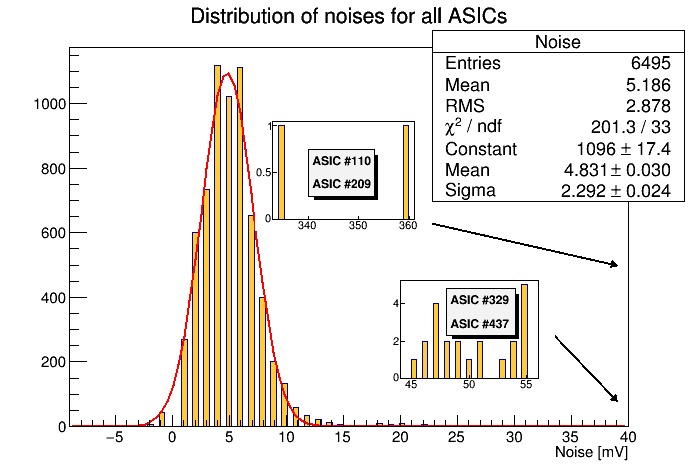
\includegraphics[width=0.5\textwidth]{./noisedist.jpg}
  \caption{Distribution of noises measured for all ASICs. Each entry represent the noise in a certain path (channel-adder-discriminator combination). The zoom-ins show the outliers.}
    \label{fig:noisedist}
\end{figure}

In figure~\ref{fig:noisedist} the total distribution of noise values is shown, having an average noise of $5.186$ mV with RMS of $2.878$ mV. Several outliers were spotted and are marked in the plot, with noises very
deviated from the mean. If we fit a gaussian profile to the distribution, the probability of having an outlier with noise over 40 mV is ~0\% and over 10 mV is less than 1\%. This outliers have been excluded
from the general characterization and calculation of the mean values.\\

No correlation of the noise between pairs of channels, adders or discriminators have been observed, so the noise is being introduced in each part of the ASIC in a similar way.\\
In figure~\ref{fig:noisech} the average noise value separated by channels and adders show that its value is pretty constant, without any outlier. 

\begin{figure}
\centering
 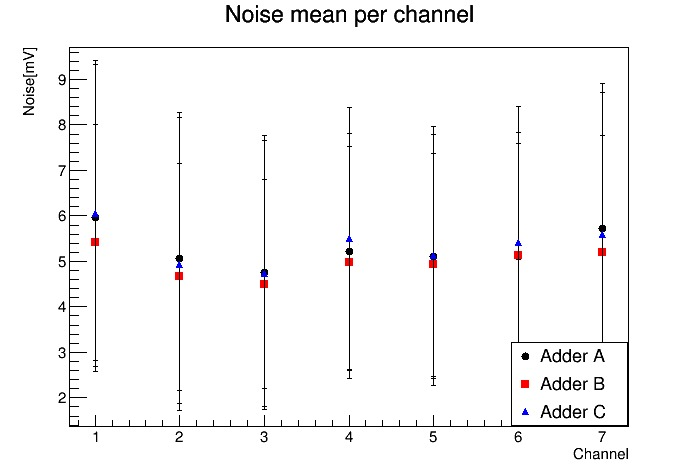
\includegraphics[width=0.5\textwidth]{./noisech.jpg}
  \caption{Noise averaged to all ASICs separated by channel and adder.}
    \label{fig:noisech}
\end{figure}


\subsection{Characterization: Summary}

\subsubsection{Gain}
The gain measured in the ASIC has a typical value of about $0,87\pm0,038$, having two channels that
slightly differ from the rest. Is the case of the channels ( 2 and 3), that for all ASICs seem to have a
deviation from the general mean, this effect is explanable by the setup configuration of the rate scan
test. There are two ASICs where gain has a very low value, under 0,7, in several of their channels.
Relative to the correlation study, there is not a strong correlation for the gain in any part of the
ASICs, having all of them a correlation coefficient below 0,5.\\

\subsubsection{Offset}
The analog offsets measured in the test have a negative mean value, while the digital offset, as the
rate scan only can provide possitive offsets, gives a positive mean value.
In the correlation plots for the analog offset, it can be observed a positive correlation between
channels , with correlation coefficients ~0,8 which means that for a high offset in one channel it is
also high in all the rest. For the adders however, the correlation observed in the plot is much lower,
and the correlation coefficient is under 0.5 , concluding that in the adders, the offset measured is
independent from each other, so they are the parts of the ASIC where the offset is introduced.
In the case of the digital offset, no correlation is observed at all, with coefficients very close to 0. It
is needed to take into account that the data of digital offset is biased by the rate scan conditions.
From the correlation plot of digital and analog offset, we can say that both offsets have a
correspondence and we are measuring the same feature, having a linear correlation with slope ~ 1.
In summary, the offset expected from a typical ASIC would be of $-6 \pm 13$ mV.

A method to calculate the offset of the ASIC in a indirect way was developed assuming a model
where the input signal and the rate scan result have a linear relation.
The offset calculated by this method have in average, a difference with the analog offset of $5,86 \pm 8$
mV.
The correlation between the fit offset and the analog offset showed that they have a linear
correlation by a factor of $0,774$.
The study of the fit offset in the different parts of the ASICs supported the idea that the adders are
responsible for introducing the offset in the ASIC.


Finally, in table(BLA) are presented the values of gain, offset and noise, averaged to all the ASICs studied. This values represent the typical values that should be expected from a 
correctly functional ASIC. If deviations from this numbers are observed, it might point to a defect in the ASIC, meaning a bad performance that won't fit the specifications. 


\section{TEST35} 
Explicar un poco el test35 para explicar el marco en que se hizo la calibracion?

\section{L1 transfer function calibration}

A method for the calibration of the L1 Analog Trigger system was developed and tested, based in a rate scan methodology. The goal of the calibration is to find the voltage threshold needed to 
obtain a trigger rate of 50\%. The calibration need to be peformed for each module of the camera and done separately for each one of the three adders of the asic and for the two discriminatos
paired to each adder. The 50\% trigger rate threshold is obtained for several input signals in order to plot a curve that allows retrieving the gain and offset of the circuit, and compare them
with the characterization of the ASICs. \\
The setup for the calibration consists on one module where a pulse with fixed amplitude and frequency can be injected in each of its seven pixels by the Slow Control Board (SCB). Increasing 
signals are generated by adding the pulses injected in each of the seven channel of the module, meaning that in total is possible to obtain up to 6 points for the calibration curve. \\
An algorithm based in a bisection method is applied to each input signal to calculate the 50\% trigger rate threshold.

\subsection{Calibration algorithm}

The algorithm for this calibration has been implemented using a scripting language specially designed for the C35 Test performed at CIEMAT integrating 35 modules in 
the mechanics of LST1 camera. It proceeds by configuring a fixed gain an frequency pulse in the SCB, in a fixed number of pixel lines. This way, the amplitude of the pulses
can be modified by adding more pixels, so each pixel added sums 1x the amplitude of the initial pulse. \\
Once the initial pulse is configured, a bisection method is used to find the 50\% trigger rate threshold. The threshold voltage in the ASIC is configured through a DAC with 8 bits, that can 
provide up to 255 different voltages from 0 to $1.2$V in steps of $4.8$mV. The algorithm initiates setting the threshold at the maximum voltage (setting the 8 bits to 1) 
and runs bit by bit, from the most significant bit, changing 1 to 0. If the new threshold voltage provide a trigger rate that is less than the target rate (in this case
the target is 50\%) then that threshold voltage is stored and the algorithm goes to the next bit. This way, only 8 steps are necessary to find the required threshold voltage.
A diagram describing the algorithm is shown in figure~\ref{fig:calalgorith}.
\begin{figure}
\centering
 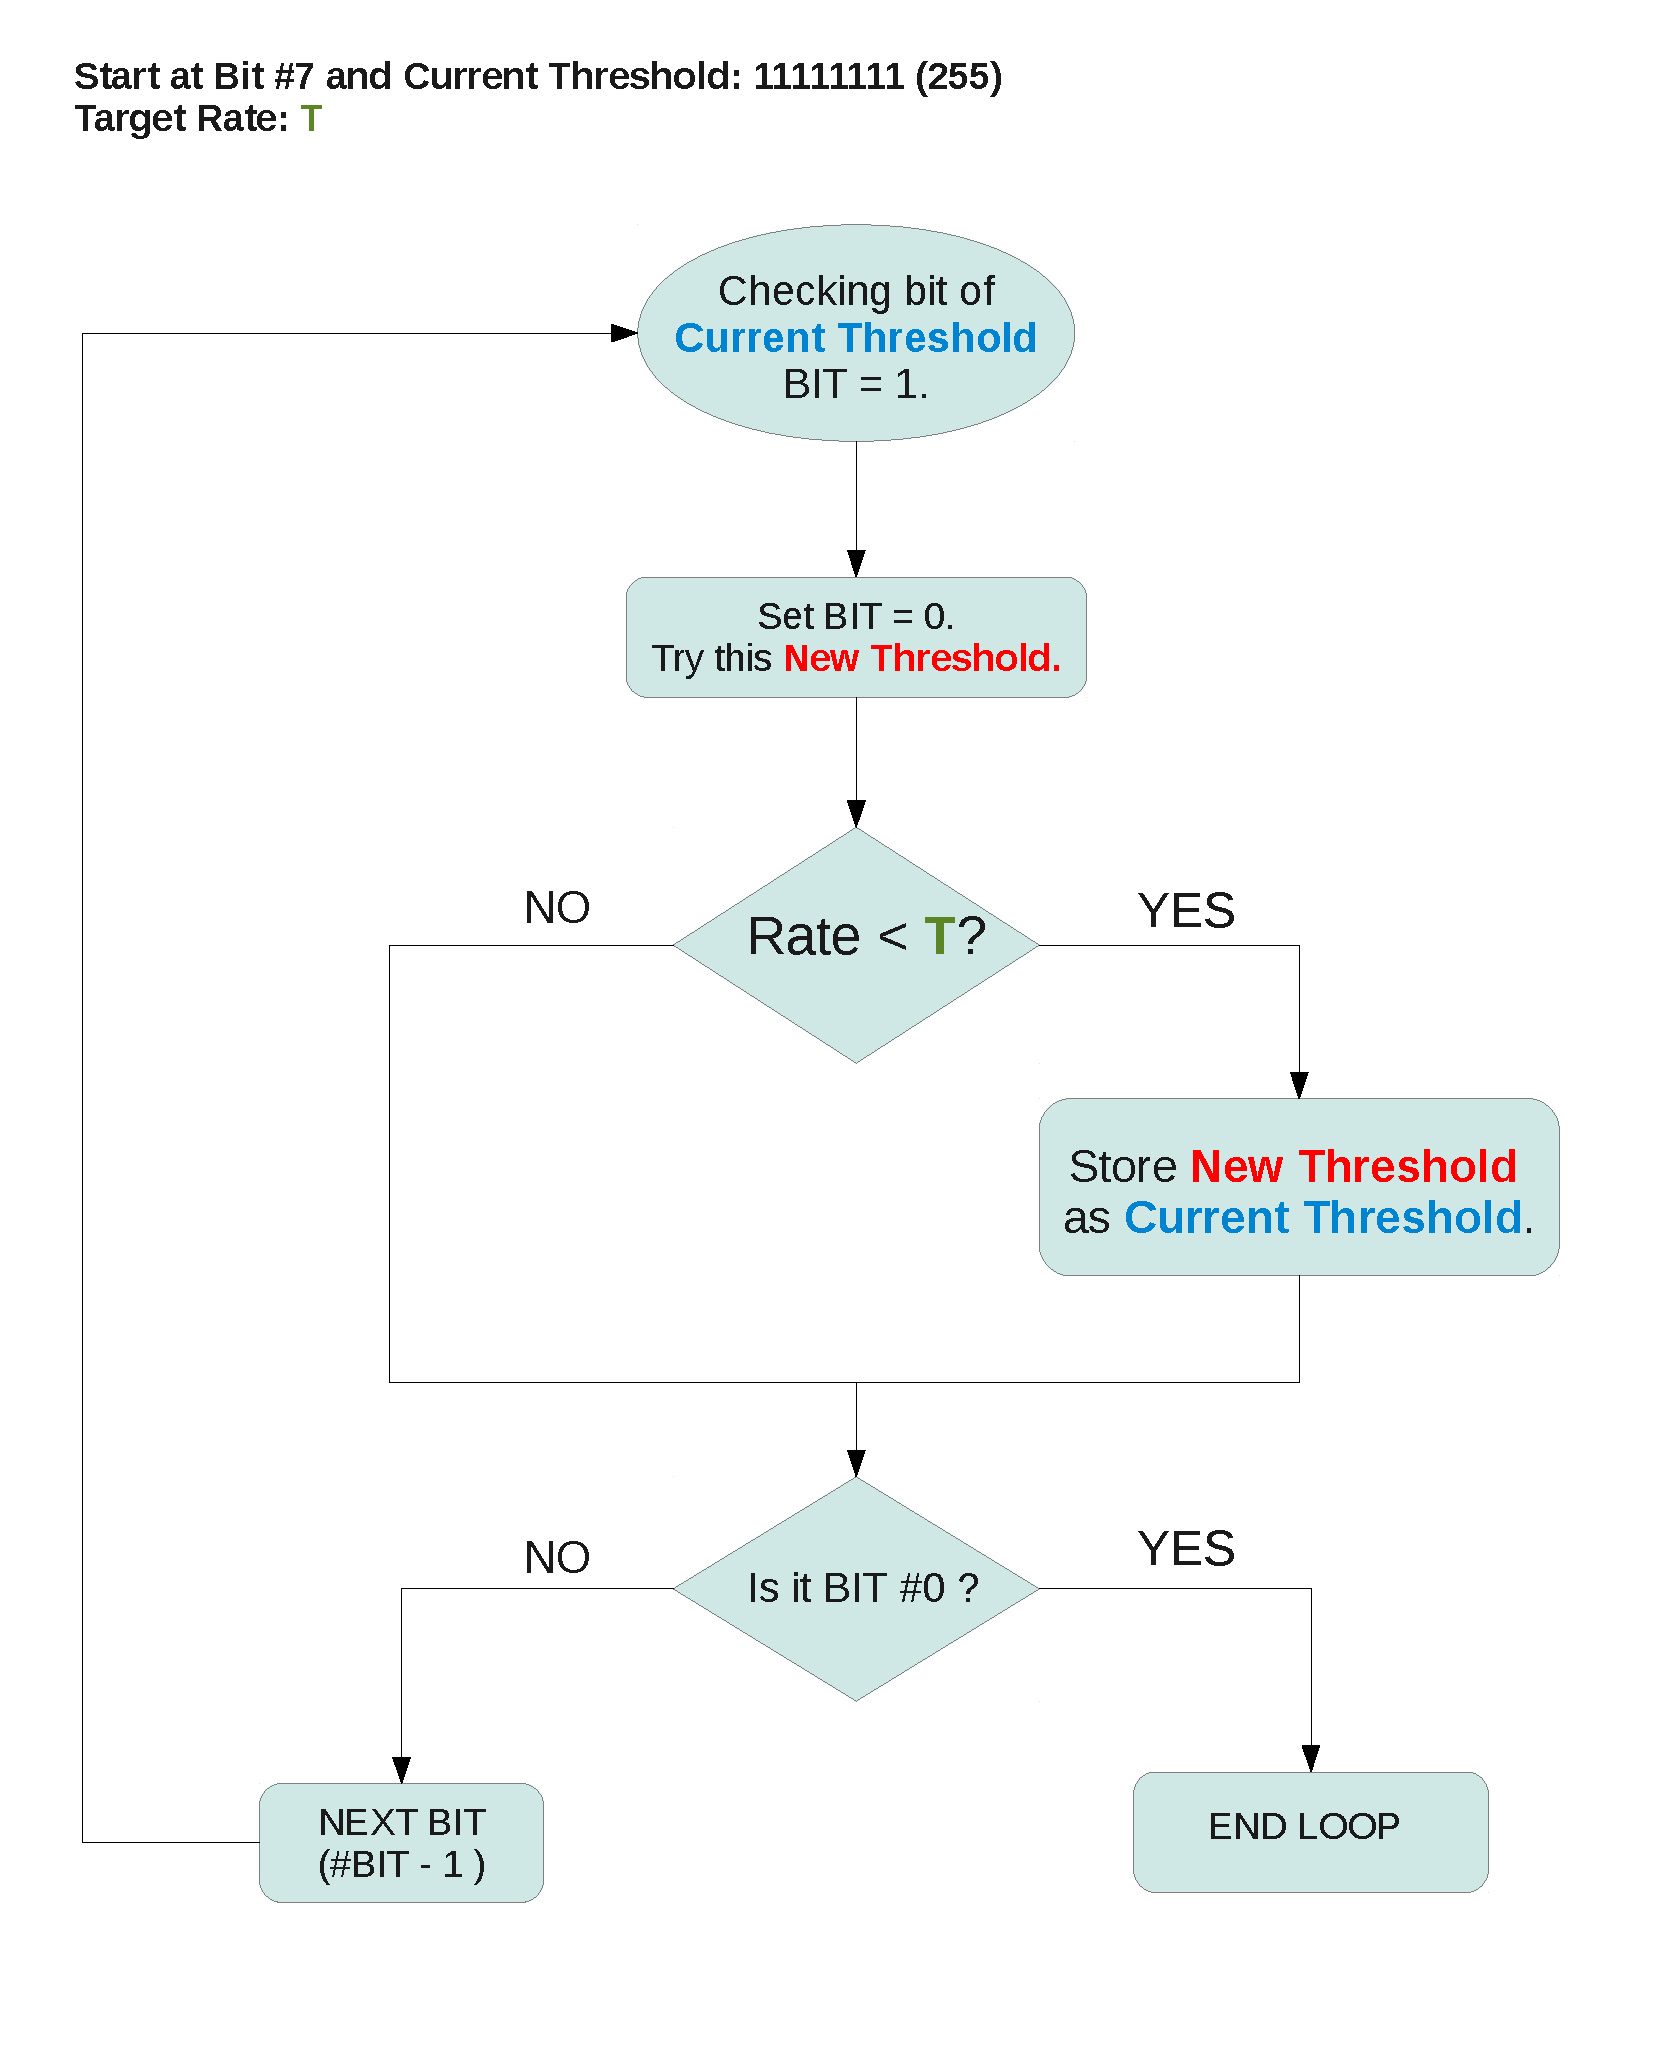
\includegraphics[width=0.5\textwidth]{./calibrationalgorithm.pdf}
  \caption{Flux diagram of the calibration algorithm.}
    \label{fig:calalgorith}
\end{figure}

Once the loop is finished, the 50\% trigger rate threshold is calculated following the formula:
\begin{equation}
50TH = \frac{(Target Rate-Baseline)}{(Baseline-Rate[Current Threshold-1]} + Current Threshold 
\end{equation}
 
Being baseline the rate at current threshold, say the last threshold that was stored in the loop. 

\subsection{Calibration result}

When the full algorithm ends and runs over the 6 possible input signals, the obtained 50\% threshold can be plotted against the number of pixels 
added to see the calibration curve (see figure ~\ref{fig:calibcurve}).

\begin{figure}
\centering
 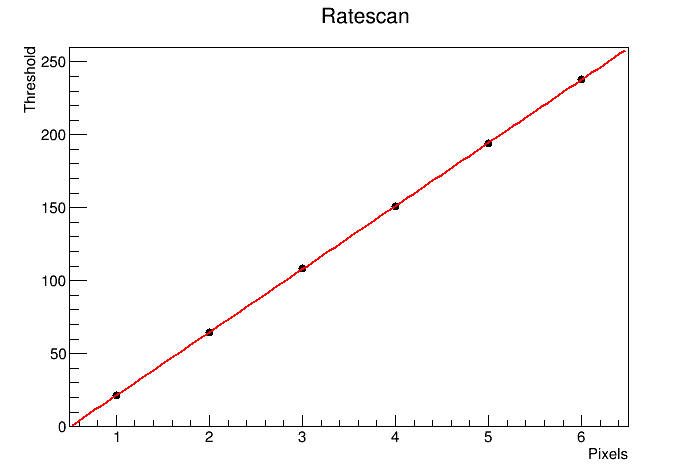
\includegraphics[width=0.5\textwidth]{./calibcurve.png}
  \caption{Result of the rate scan for Adder A of one module}
    \label{fig:calibcurve}
\end{figure}

If the initial pulse injected by the SCB is known and assuming that the adding is correct, the amplitude of each pulse is simply the multiplication of the initial pulse by the number
of pixels added, being possible to obtain the gain and offset of the asic. 

\end{document}
